\documentclass[12pt]{article}
\usepackage[
backend=biber,
style=abnt,
sorting=nyt
]{biblatex}
\usepackage{csquotes}
\addbibresource{bibliografia.bib}
\AtBeginBibliography{\raggedright \footnotesize}
\setlength{\bibitemsep}{\baselineskip}

\usepackage{amsmath} %Para usar símbolos matemáticos

\usepackage[brazil]{babel} %Para usar a linguagem português
\addto\captionsbrazil{
    \renewcommand{\contentsname}{\texorpdfstring{\normalsize SUMÁRIO}{SUMÁRIO}}
    \renewcommand{\listtablename}{\texorpdfstring{\normalsize ÍNDICE DE TABELAS}{ÍNDICE DE TABELAS}}
    \renewcommand{\listfigurename}{\texorpdfstring{\normalsize ÍNDICE DE FIGURAS}{ÍNDICE DE FIGURAS}}
}

\usepackage{subcaption}
\usepackage{float}
\usepackage{graphicx} %Para inserir imagens
\usepackage{geometry} %Para alterar propriedades da página
\geometry{
a4paper,
left=30mm,
top=30mm,
right=20mm,
bottom=20mm
}

\usepackage[hidelinks]{hyperref}

\usepackage{tocloft}
\renewcommand{\cfttoctitlefont}{\hfill}
\renewcommand{\cftaftertoctitle}{\hfill}
\renewcommand{\cftsecfont}{\normalsize\normalfont\bfseries}
\renewcommand{\cftsubsecindent}{0pt}
\renewcommand{\cftsubsecfont}{\normalsize\normalfont}
\renewcommand{\cftsubsubsecindent}{0pt}
\renewcommand{\cftsubsubsecfont}{\normalsize\normalfont\bfseries}
\renewcommand{\cftsecleader}{\cftdotfill{\cftdotsep}}
\renewcommand{\cftlottitlefont}{\hfill} %Centralizar o título da lista de tabelas
\renewcommand{\cftafterlottitle}{\hfill}
\renewcommand{\cfttabpresnum}{Tabela\ } %Adicionar Tabela antes do nome de cada item
\renewcommand{\cfttabaftersnum}{:\ }
\setlength{\cfttabnumwidth}{4.75em}
\renewcommand{\cftdotsep}{1}
\renewcommand{\cftloftitlefont}{\hfill}
\renewcommand{\cftafterloftitle}{\hfill}
\renewcommand{\cftfigpresnum}{Figura\ }
\renewcommand{\cftfigaftersnum}{:\ }
\setlength{\cftfignumwidth}{4.75em}

\usepackage{titlesec}
\titleformat{\section}{\normalsize\bfseries\MakeUppercase}{\thesection}{0.5em}{}
\titleformat{\subsection}{\normalsize\MakeUppercase}{\thesubsection}{0.5em}{}
\titleformat{\subsubsection}{\normalsize\bfseries}{\thesubsubsection}{0.5em}{}

\usepackage{fancyhdr}
\pagestyle{fancy}
\fancyhf{} % Limpa os cabeçalhos e rodapés
\fancyhead[R]{\footnotesize\thepage} % Coloca o número da página no canto superior direito
\fancyfoot[C]{} % Remove qualquer número de página no rodapé
\renewcommand{\headrulewidth}{0pt} % Remove a linha horizontal do cabeçalho
\renewcommand{\footrulewidth}{0pt} % Remove a linha horizontal do rodapé

\usepackage{multicol}
\usepackage{pgfplots}
\pgfplotsset{compat=1.18}
\usepackage[american]{circuitikz}
\usetikzlibrary{external}\tikzexternalize
\usetikzlibrary{positioning}

\usepackage{setspace} %Para alterar o espaçamento das linhas
\setstretch{1.5}

\begin{document}
    \begin{titlepage}
    \begin{center}
        \large
        Universidade Federal do Espírito Santo - UFES\\
        Departamento de Computação e Eletrônica - DCEL\\
        Engenharia de Computação
        
        \vfill
        \textbf{
        Relatório da experiência 01\\
        Resistores\\~\\
        }
        
        Disciplina: Circuitos Elétricos I\\
        Prof. Flávio Duarte Couto Oliveira\\
        
        \vfill
        \begin{flushright}
            Pedro Henrique Alves do Nascimento
        \end{flushright}
        
        \vfill
        Espírito Santo\\
        Dezembro 2024
    \end{center}
    \newpage
\end{titlepage}
    
    \listoftables
    \thispagestyle{empty}
    \newpage

    \listoffigures
    \thispagestyle{empty}
    \newpage

    \tableofcontents
    \thispagestyle{empty}
    \newpage

    \section*{Pedro Henrique Alves do Nascimento}
    \section{INTRODUÇÃO TEÓRICA}
    \subsection{LEI DE OHM}
    A lei de Ohm é a relação algébrica entre corrente tensão para um resistor \parencite[][, p. 32]{nilsson}, dada pela Equação \ref{lei-de-ohm}
    \begin{equation}
        V=R\times i \label{lei-de-ohm}
    \end{equation}
    onde $V$ é a tensão, em Volts (V) nos terminais do resistor, $R$ é a resistência elétrica do resistor, em Ohms ($\Omega$) e $i$ a corrente que passa pelo resistor, em Ampères (A).

    Ou seja, traçando-se um gráfico de tensão $\times$ corrente para um resistor ôhmico, tem-se uma função linear, onde $\tan{\alpha}=\frac{V'}{i'}$ é a resistência $R$ daquele resistor, como mostrado na Figura \ref{fig:resistorohmico}.
        \begin{figure}[h!]
            \centering
            \caption{Gráfico $V\times i$ de um resistor ôhmico.}
            \begin{minipage}{0.5\textwidth}
                \centering
                \begin{tikzpicture}
                    \begin{axis}[
                        axis lines=middle,
                        xlabel={$i$},
                        ylabel={$V$},
                        xmin=-0.5, xmax=3,
                        ymin=-0.5, ymax=3,
                        xtick={1.15},
                        xticklabel={$i'$},
                        ytick={2},
                        yticklabel={$V'$}
                    ]
                    \addplot[
                        thick,
                        domain=0:2,
                        samples=5,
                    ] {sqrt(3)*x};
                    \draw[smooth, thick] (0.5,0) arc (0:60:0.5) node[midway] {$\alpha$};
                    \node at (axis cs:0,0) [anchor=north east] {$0$};
                    \draw[dashed, color=gray!50] (0,2) -- (1.15,2) -- (1.15,0);
                    \end{axis}
                \end{tikzpicture}

                \raggedright \footnotesize Fonte: Elaborado pelo autor.
                \label{fig:resistorohmico}
            \end{minipage}
        \end{figure}
    
    \subsection{RESISTORES}
    Resistores são componentes eletrônicos fundamentais, projetados para limitar o fluxo de corrente elétrica em um circuito, convertendo parte dessa energia em calor. Estes dispositivos são tipicamente feitos de materiais com alta resistividade, como carbono ou filme metálico. Dependendo de suas propriedades, os resistores podem ser classificados em fixos, cuja resistência é constante, e variáveis, cuja resistência pode ser ajustada conforme necessário.
    
    \subsubsection{Aplicações práticas dos resistores}
    Um uso comum dos resistores é se comportar como divisor de tensão, onde resistores conectados em série distribuem a tensão de uma fonte entre seus terminais de acordo com seus valores de resistência. Esse comportamento é ilustrado na Figura \ref{fig:divisor-tensao}.

    De acordo com a Lei de Ohm, a tensão em cada resistor de um divisor de tensão é proporcional à sua resistência. Quanto maior a resistência de um resistor, maior será a tensão sobre ele. Esse fenômeno é descrito pela Equação \ref{eq:divisor-de-tensao}, derivada diretamente da Lei de Ohm aplicada ao circuito. Por exemplo, se um elemento for conectado aos terminais de \(R_1\), ele estará sujeito à tensão \(v_1\) \parencite[][, p. 65]{nilsson}. 
    
    \begin{figure}[H]
        \centering
        \caption{Circuito divisor de tensão.}
        \begin{tikzpicture}
            \draw (-0.5,0) to [short] (2,0) to
            [short] (2,0.5) to
            [R, l=$R_2$, v<=$v_2$] (2,1.5) to
            [short] (2,2.5) to
            [R, l=$R_1$, v<=$v_1$] (2,3.5) to
            [short] (2,4) to
            [short] (-0.5,4) to
            [voltage source, l_=$v_s$, sources/scale=1.5] (-0.5,0);
        \end{tikzpicture}
        \label{fig:divisor-tensao}
    \end{figure}

    \begin{equation}
        v_1=v_s\times\frac{R_1}{R_1+R_2} \text{\hspace{1.5cm} e\hspace{1.5cm}} v_2=v_s\times\frac{R_2}{R_1+R_2}
        \label{eq:divisor-de-tensao}
    \end{equation}
    
    Outra aplicação importante dos resistores é o divisor de corrente, que ocorre quando dois resistores estão conectados em paralelo a uma fonte de corrente. Nesse caso, o resistor de menor resistência conduz proporcionalmente a maior parte da corrente, de acordo com a Lei de Ohm e a Lei de Kirchhoff das Correntes \parencite[][, p. 66]{nilsson}.
    
    A Figura \ref{fig:divisor-corrente} ilustra o circuito em questão, enquanto a Equação \ref{eq:divisor-de-corrente} descreve a corrente que passa por cada resistor.

    \begin{figure}[H]
        \centering
        \caption{Circuito divisor de corrente.}
        \begin{tikzpicture}
            \ctikzset{nodes width=0.05};
            \draw (0,0) to [short, -*] (4,0) to
            [short] (4,1) to
            [R, l=$R_1$] (4,2) to
            [short, -*] (4,3) to
            [short] (0,3) to
            [current source, l_=$i_s$, invert, sources/scale=1.5] (0,0);
            \draw (4.2,0) to [open, f<_=$i_1$] (4.2,3);
            \draw (4,0) to [short] (6,0) to
            (6,1) [short] to
            [R, l=$R_2$] (6,2) to
            [short] (6,3) to
            [short] (4,3);
            \draw (6.2,0) to [open, f<_=$i_2$] (6.2,3);
        \end{tikzpicture}
        \label{fig:divisor-corrente}
    \end{figure}

    \begin{equation}
        i_1=i_s\times\frac{R_2}{R_1+R_2}\text{\hspace{1.5cm} e\hspace{1.5cm}}i_2=i_s\times\frac{R_1}{R_1+R_2}
        \label{eq:divisor-de-corrente}
    \end{equation}

    \subsubsection{Resistores Fixos}
    Os resistores fixos possuem características como valor nominal e tolerância, que são identificados por meio de uma tabela de cores.
    
    Essa convenção para as cores utilizadas foi introduzida na década de 1920 pela Radio Manufacturers Association (RMA), posteriormente adotada e mantida pelo International Electrotechnical Commission (IEC). O sistema é útil para permitir uma rápida identificação em resistores muito pequenos, onde a impressão de números seria inviável.

    Cada cor na tabela corresponde a um valor específico, facilitando a identificação e a seleção do resistor adequado para uma aplicação particular. A Tabela \ref{tab:corResist} e a Figura \ref{fig:resistor} ilustram o processo de codificação por cores e a representação de um resistor com suas faixas.
    
    \begin{figure}[H]
        \centering
        \caption{Resistor e suas faixas.}
        \begin{tikzpicture}[scale=2]
            \draw[thick] (-1,0.5) rectangle (1,-0.5);
            \draw[fill=gray] (-1.5,0.1) rectangle (-1,-0.1); 
            \draw[fill=gray] (1,0.1) rectangle (1.5,-0.1);
            \definecolor{auburn}{rgb}{0.43, 0.21, 0.1}
            \draw[fill=auburn] (-0.8,0.5) rectangle (-0.6,-0.5);
            \draw[fill=black] (-0.4,0.5) rectangle (-0.2,-0.5);
            \draw[fill=orange] (0,0.5) rectangle (0.2,-0.5);
            \draw[fill=yellow] (0.6,0.5) rectangle (0.8,-0.5);
            
            \draw[thick, <-] (-0.7,-0.5) -- (-0.7,-1);
            \draw[thick] (-0.7, -1) -- (-1.2,-1) node[left] {1º dígito};
            \draw[thick, <-] (-0.3,-0.5) -- (-0.3,-1.3);
            \draw[thick] (-0.3, -1.3) -- (-1.2,-1.3) node[left] {2º dígito};
            \draw[thick, <-] (0.1,-0.5) -- (0.1,-1.6);
            \draw[thick] (0.1, -1.6) -- (-1.2,-1.6) node[left] {Multiplicador};
            \draw[thick, <-] (0.7,-0.5) -- (0.7,-1.9);
            \draw[thick] (0.7, -1.9) -- (-1.2,-1.9) node[left] {Tolerância};
            \draw (-2.55, -2.2) node[right] {\footnotesize{Fonte: Elaborado pelo autor.}};
        \end{tikzpicture}
        \label{fig:resistor}
    \end{figure}

    \begin{table}[H]
        \caption{Tabela do cores dos resistores fixos.}
        \label{tab:corResist}
        \centering
        % \vspace{0.5em}
        \setstretch{1.5}{
        \begin{tabular}{ccclc}
        \hline
        Cor & 1ª Faixa & 2ª Faixa & Multiplicador ($\Omega$) & Tolerância\\
        \hline Preto & 0 & 0 & $\times 1$ & \\
        Marrom & 1 & 1 & $\times 10$ & $\pm$ 1\%\\
        Vermelho & 2 & 2 & $\times 100$ & $\pm$ 2\%\\
        Laranja & 3 & 3 & $\times 1$ k & \\
        Amarelo & 4 & 4 & $\times 10$ k & \\
        Verde & 5 & 5 & $\times 100$ k & $\pm$ 0.5\%\\
        Azul & 6 & 6 & $\times 1$ M & $\pm$ 0.25\%\\
        Violeta & 7 & 7 & $\times 10$ M & $\pm$ 0.1\%\\
        Cinza & 8 & 8 & & $\pm$ 0.05\%\\
        Branco & 9 & 9 & & \\
        Dourado & & & $\times 0.1$ & $\pm$ 5\%\\
        Prateado & & & $\times 0.01$ & $\pm$ 10\%\\
        \hline
        \end{tabular}}\\
        \footnotesize Fonte: blog.fazedores.com (Adaptado)\nocite{codigo_cores_resistores}.
    \end{table}

    \subsubsection{Resistores Variáveis}
    Os resistores variáveis, como os potenciômetros, são componentes com três terminais. A resistência é ajustada movendo o terminal central em relação aos terminais externos. A resistência máxima é obtida quando o terminal central é posicionado na posição 3 da Figura \ref{fig:potenciometro}.
    
    O funcionamento desses resistores se baseia na variação do comprimento do segmento resistivo. De acordo com a equação $R = \rho\times\frac{L}{A}$ --- onde $R$ é a resistência do material, $\rho$ a sua resistividade, $L$ o comprimento e $A$ a área da seção transversal --- a resistência é diretamente proporcional ao comprimento do resistor.
    
    Assim, quanto mais próximo o terminal central estiver da posição 3, maior será a resistência. A Figura \ref{fig:potenciometro} exemplifica o uso de um potenciômetro em sua representação gráfica.

    Resistores variáveis são amplamente utilizados em dispositivos como controles de volume em equipamentos de áudio, nos quais a resistência ajusta a tensão, afetando diretamente a saída do som.

    \begin{figure}[H]
        \centering
        \caption{Representação gráfica de potenciômetro.}
        \begin{minipage}{0.4\textwidth}
            \centering
            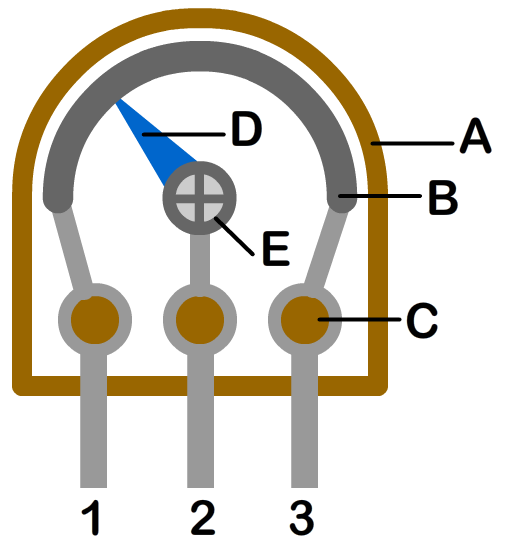
\includegraphics[width=\textwidth]{external-figures/resistor-variavel.png}
            \raggedright \footnotesize Fonte: ricardoteix.com (2021)\nocite{ricardo_teix}.
            \label{fig:potenciometro}
        \end{minipage}
    \end{figure}

    \begin{figure}[H]
        \centering
        \caption{Representação de resistor fixo e variável em um circuito.}
        \begin{tikzpicture}
            \draw (-0.5,0) -- (0,0) to [R, label=$R$] (1,0) -- (1.5,0) to
            [open] (2.5,0) -- (3,0) to
            [vR, l=$R_{var}$] (4,0) -- (4.5,0);
        \end{tikzpicture}
    \end{figure}
    
    \subsection{OHMÍMETRO}
    O ohmímetro é um dispositivo para a medição da resistência elétrica. Para realizar a medição, o ohmímetro deve ser conectado em paralelo com o resistor e não deve ser exposto a nenhuma tensão externa, pois o aparelho funciona fornecendo uma corrente ao resistor e medindo a tensão entre seus terminais \parencite{ohmmeter_website}.
    
    A partir dessa medição, é possível calcular a resistência utilizando a Lei de Ohm. Caso haja uma fonte de tensão adicional no circuito, a medição poderá ser afetada, uma vez que a tensão nos terminais do resistor será influenciada pela presença dessa fonte. A Figura \ref{fig:ohmimetro} ilustra o esquema de ligação do ohmímetro.
    \begin{figure}[H]
        \centering
        \caption{Esquema de ligação de um ohmímetro.}
        \begin{minipage}{0.5\textwidth}
            \centering
            \begin{tikzpicture}
                \draw (-0.5,0) -- (0,0) to [R, l=$R$] (3,0) to
                [short, *-] (3,2) to
                [rmeterwa, t=$\Omega$] (0,2) to
                [short, -*] (0,0);
                \draw (3,0) -- (3.5,0);
            \end{tikzpicture}
            \label{fig:ohmimetro}
        \end{minipage}
    \end{figure}

\section{PRÁTICA EM LABORATÓRIO}
\subsection{PARTE 1}
Primeiramente, foram identificados 10 resistores com base na cor de cada uma de suas faixas  e anotou-se seus valores nominais e tolerâncias.

Após isso, mediu-se a resistência de cada resistor com um multímetro na escala de resistência e anotou-se os valores medidos. Então, calculou-se o erro utilizando a Equação \ref{eq:erro}:
\begin{equation}
    Erro(\%) = \left(\frac{R_{medido}}{R_{nominal}} -1\right)\times 100\%
    \label{eq:erro}
\end{equation}

As medições e erros calculados estão contidos na Tabela \ref{tab:erro_resistores}.
\begin{table}[H]
    \caption{Valores e nominais e erro de medição dos resistores.}
    \label{tab:erro_resistores}
    \centering
    \setstretch{1.5}{
    \begin{tabular}{ccccc}
        \hline Resistor & Valor nominal ($\Omega$) & Tolerância (\%) & Valor medido ($\Omega$) & Erro (\%) \\
        \hline $R_1$    & 47 k                     & $\pm$5          & 46,3 k                  & -1,49     \\
        $R_2$           & 22 k                     & $\pm$5          & 21,6 k                  & -1,82     \\
        $R_3$           & 5,6 k                    & $\pm$5          & 5,48 k                  & -2,14     \\
        $R_4$           & 22                       & $\pm$5          & 21,5                    & -2,27     \\
        $R_5$           & 10 k                     & $\pm$5          & 9,88 k                  & -1,20     \\
        $R_6$           & 3,9 k                    & $\pm$5          & 3,88 k                  & -0,51     \\
        $R_7$           & 150                      & $\pm$5          & 150                     & 0,00      \\
        $R_8$           & 27 k                     & $\pm$5          & 26,77 k                 & -0,85     \\
        $R_9$           & 3,3 k                    & $\pm$5          & 3,25 k                  & -1,52     \\
        $R_{10}$        & 1,2 k                    & $\pm$5          & 1,18 k                  & -1,67     \\
        \hline
    \end{tabular}}\\
    \footnotesize{Fonte: Elaborado pelo autor.}
\end{table}

\begin{figure}[H]
    \centering
    \caption{Resistores utilizados na parte 1.}
    \begin{minipage}{0.45\textwidth}
        \centering
        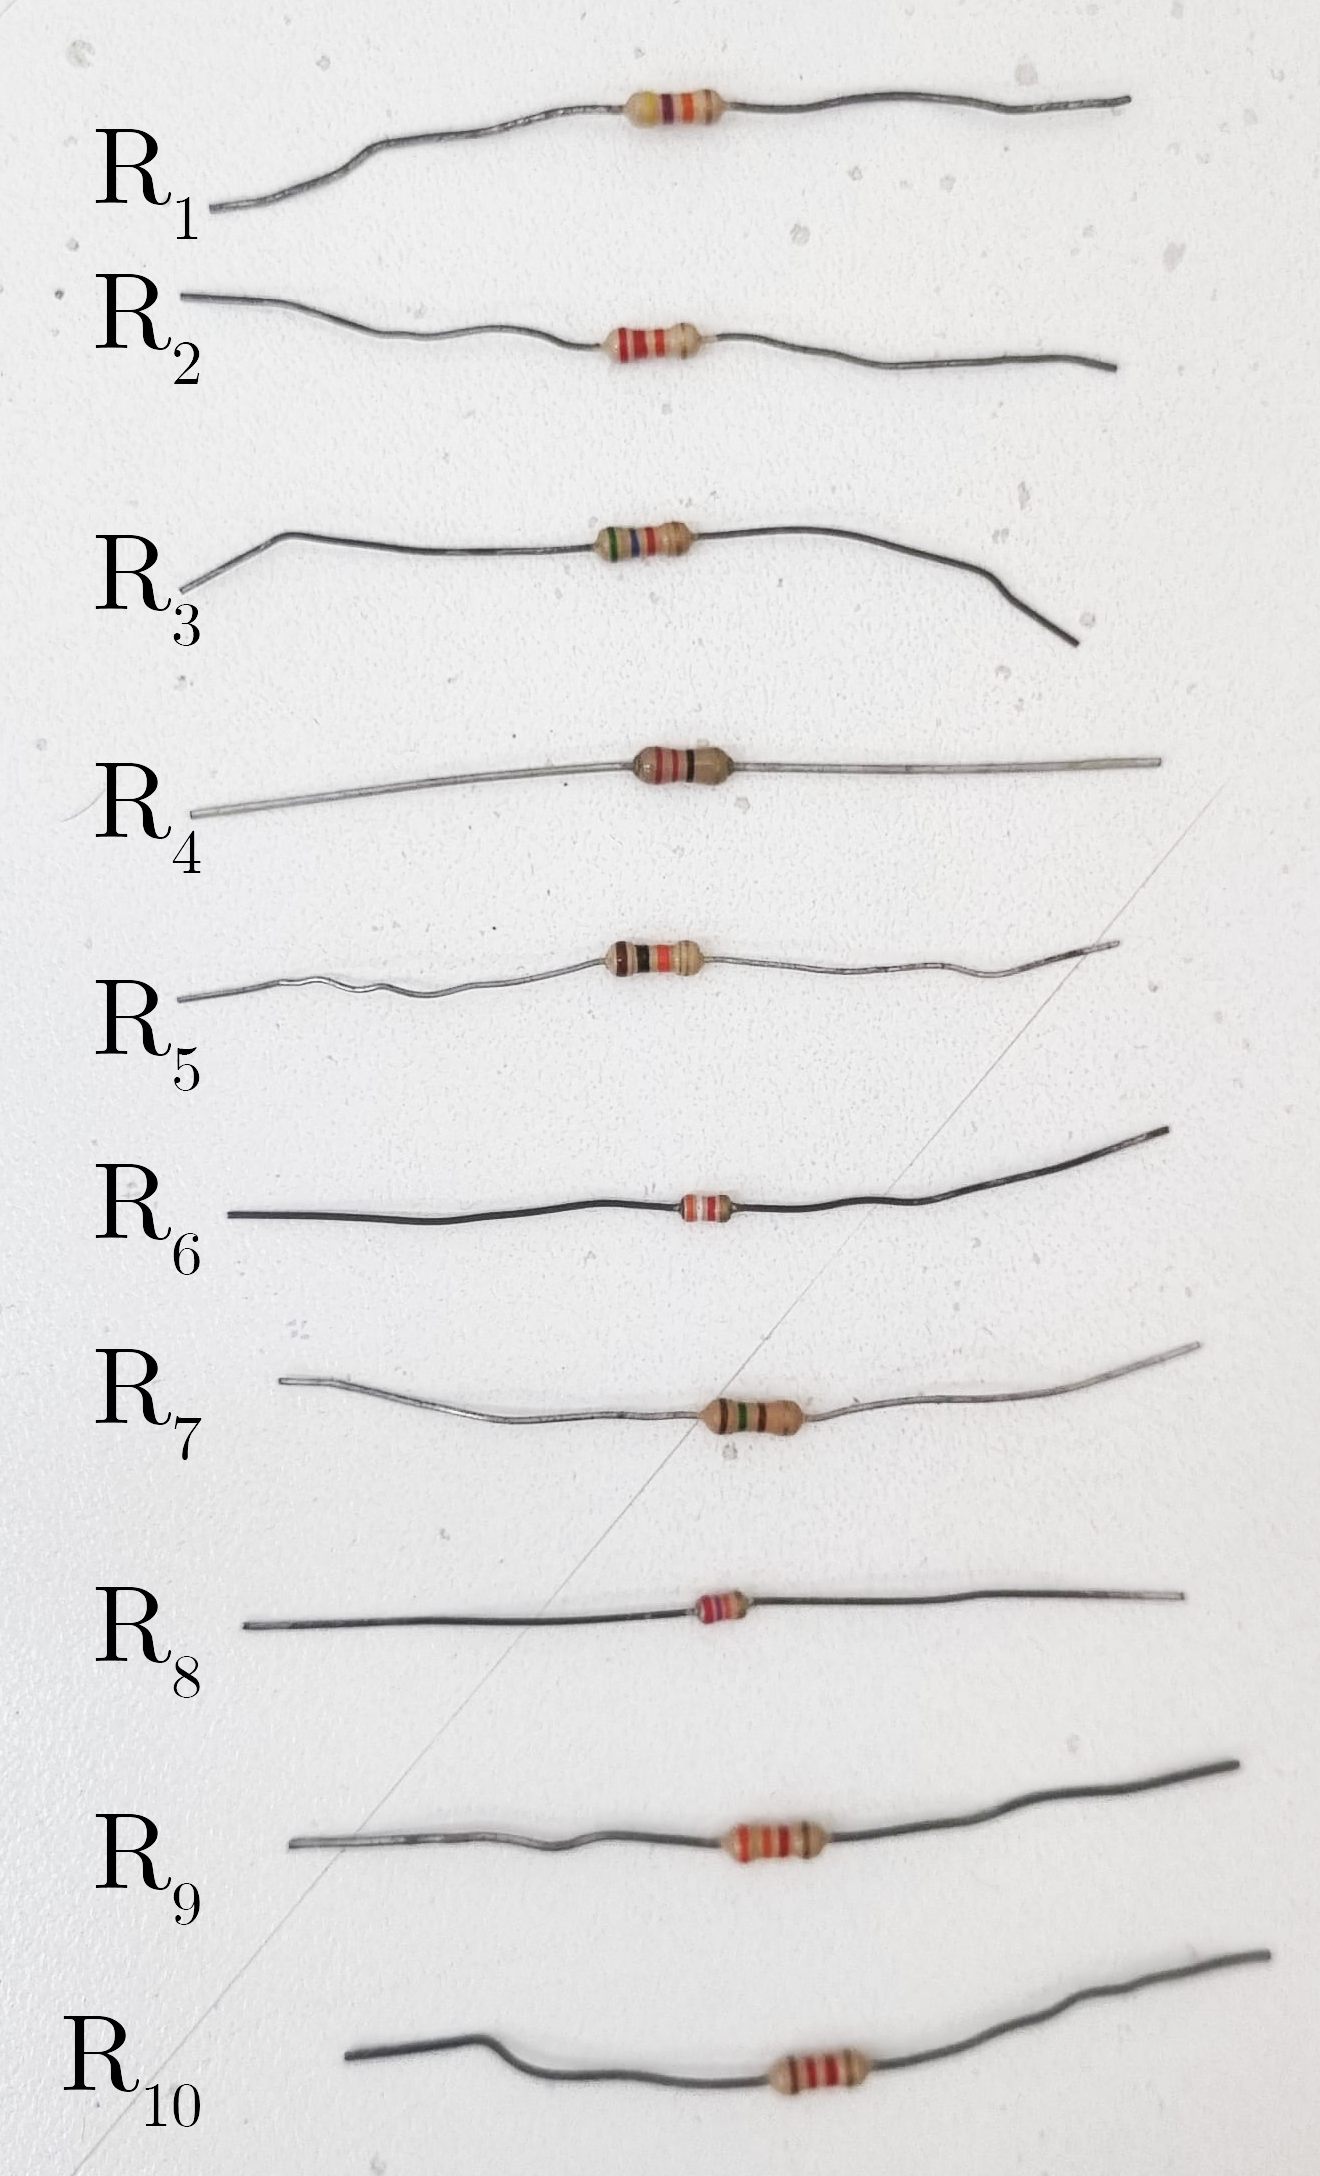
\includegraphics[width=\textwidth]{external-figures/resistores-pratica1.png}\\
        \raggedright\footnotesize{Fonte: Elaborado pelo autor.}
        \label{fig:pratica1}
    \end{minipage}
\end{figure}

\subsection{PARTE 2}
A segunda parte teve como objetivo mostrar a relação entre corrente e tensão de um resistor conforme a tensão varia.

Para isso, foi utilizado um multímetro, uma fonte variável utilizada na faixa de 0 V a 12 V e quatro resistores com resistências de 1 k$\Omega$ a 50 k$\Omega$, mostrados na Figura \ref{fig:pratica2}.

\begin{figure}[H]
    \centering
    \caption{Resistores utilizados na parte 2.}
    \begin{minipage}{0.45\textwidth}
        \centering
        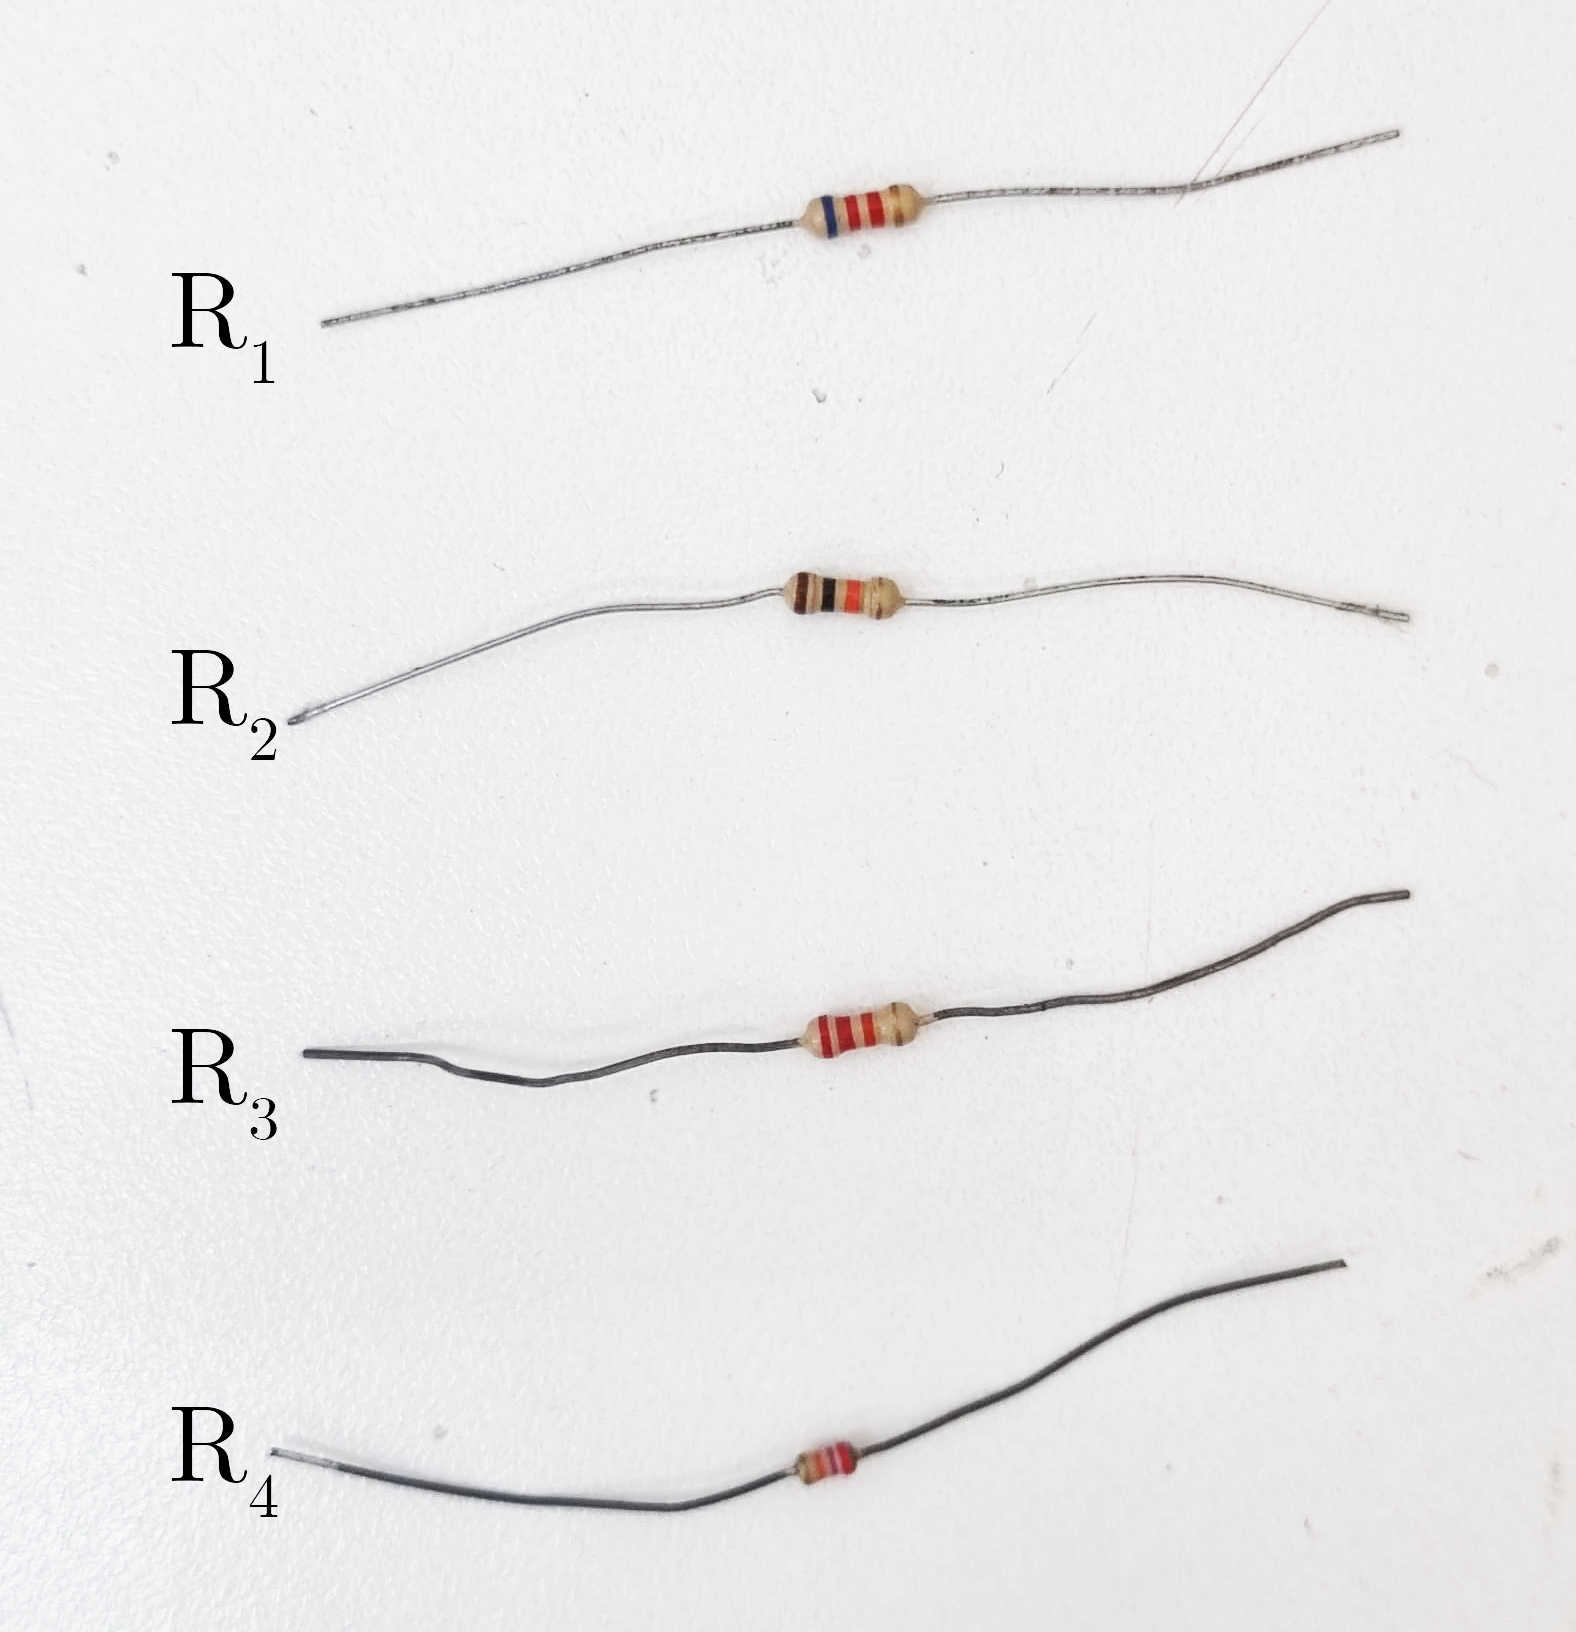
\includegraphics[width=\textwidth]{external-figures/resistores-pratica2.png}\\
        \raggedright\footnotesize{Fonte: Elaborado pelo autor.}
        \label{fig:pratica2}
    \end{minipage}
\end{figure}

Primeiramente, foi montado o circuito conforme a Figura \ref{fig:pratica-parte2}, a fonte foi ajustada para permitir uma corrente máxima de 0,36 A (inferior ao máximo que o multímetro em questão suporta).

\begin{figure}[H]
    \centering
    \caption{Circuito da parte 2 da aula prática.}
    \begin{subfigure}{0.45\textwidth}
        \centering
        \caption{Em esquema.}
        \begin{tikzpicture}
            \tikzset{vmeter/.style={rmeterwa, t=V}}
            \tikzset{ameter/.style={rmeterwa, t=A}}
            \draw (0,0) to [short] (3,0) to
            [short] (5,0) to
            [vmeter] (5,3) to
            [short] (3,3) to
            [ameter, t=mA] (0,3) to
            [battery1, l_=$E$, name=battery] (0,0);
            \ctikztunablearrow{2}{1}{-210}{battery};
            \draw (0,1.5) node[below right] {\small$-$}
            (0,1.5) node[above right] {\small$+$};
            \draw (3,0) to [R, l=$R$] (3,3);
        \end{tikzpicture}
    \end{subfigure}
    \hfill
    \begin{subfigure}{0.45\textwidth}
        \centering
        \caption{No laboratório.}
        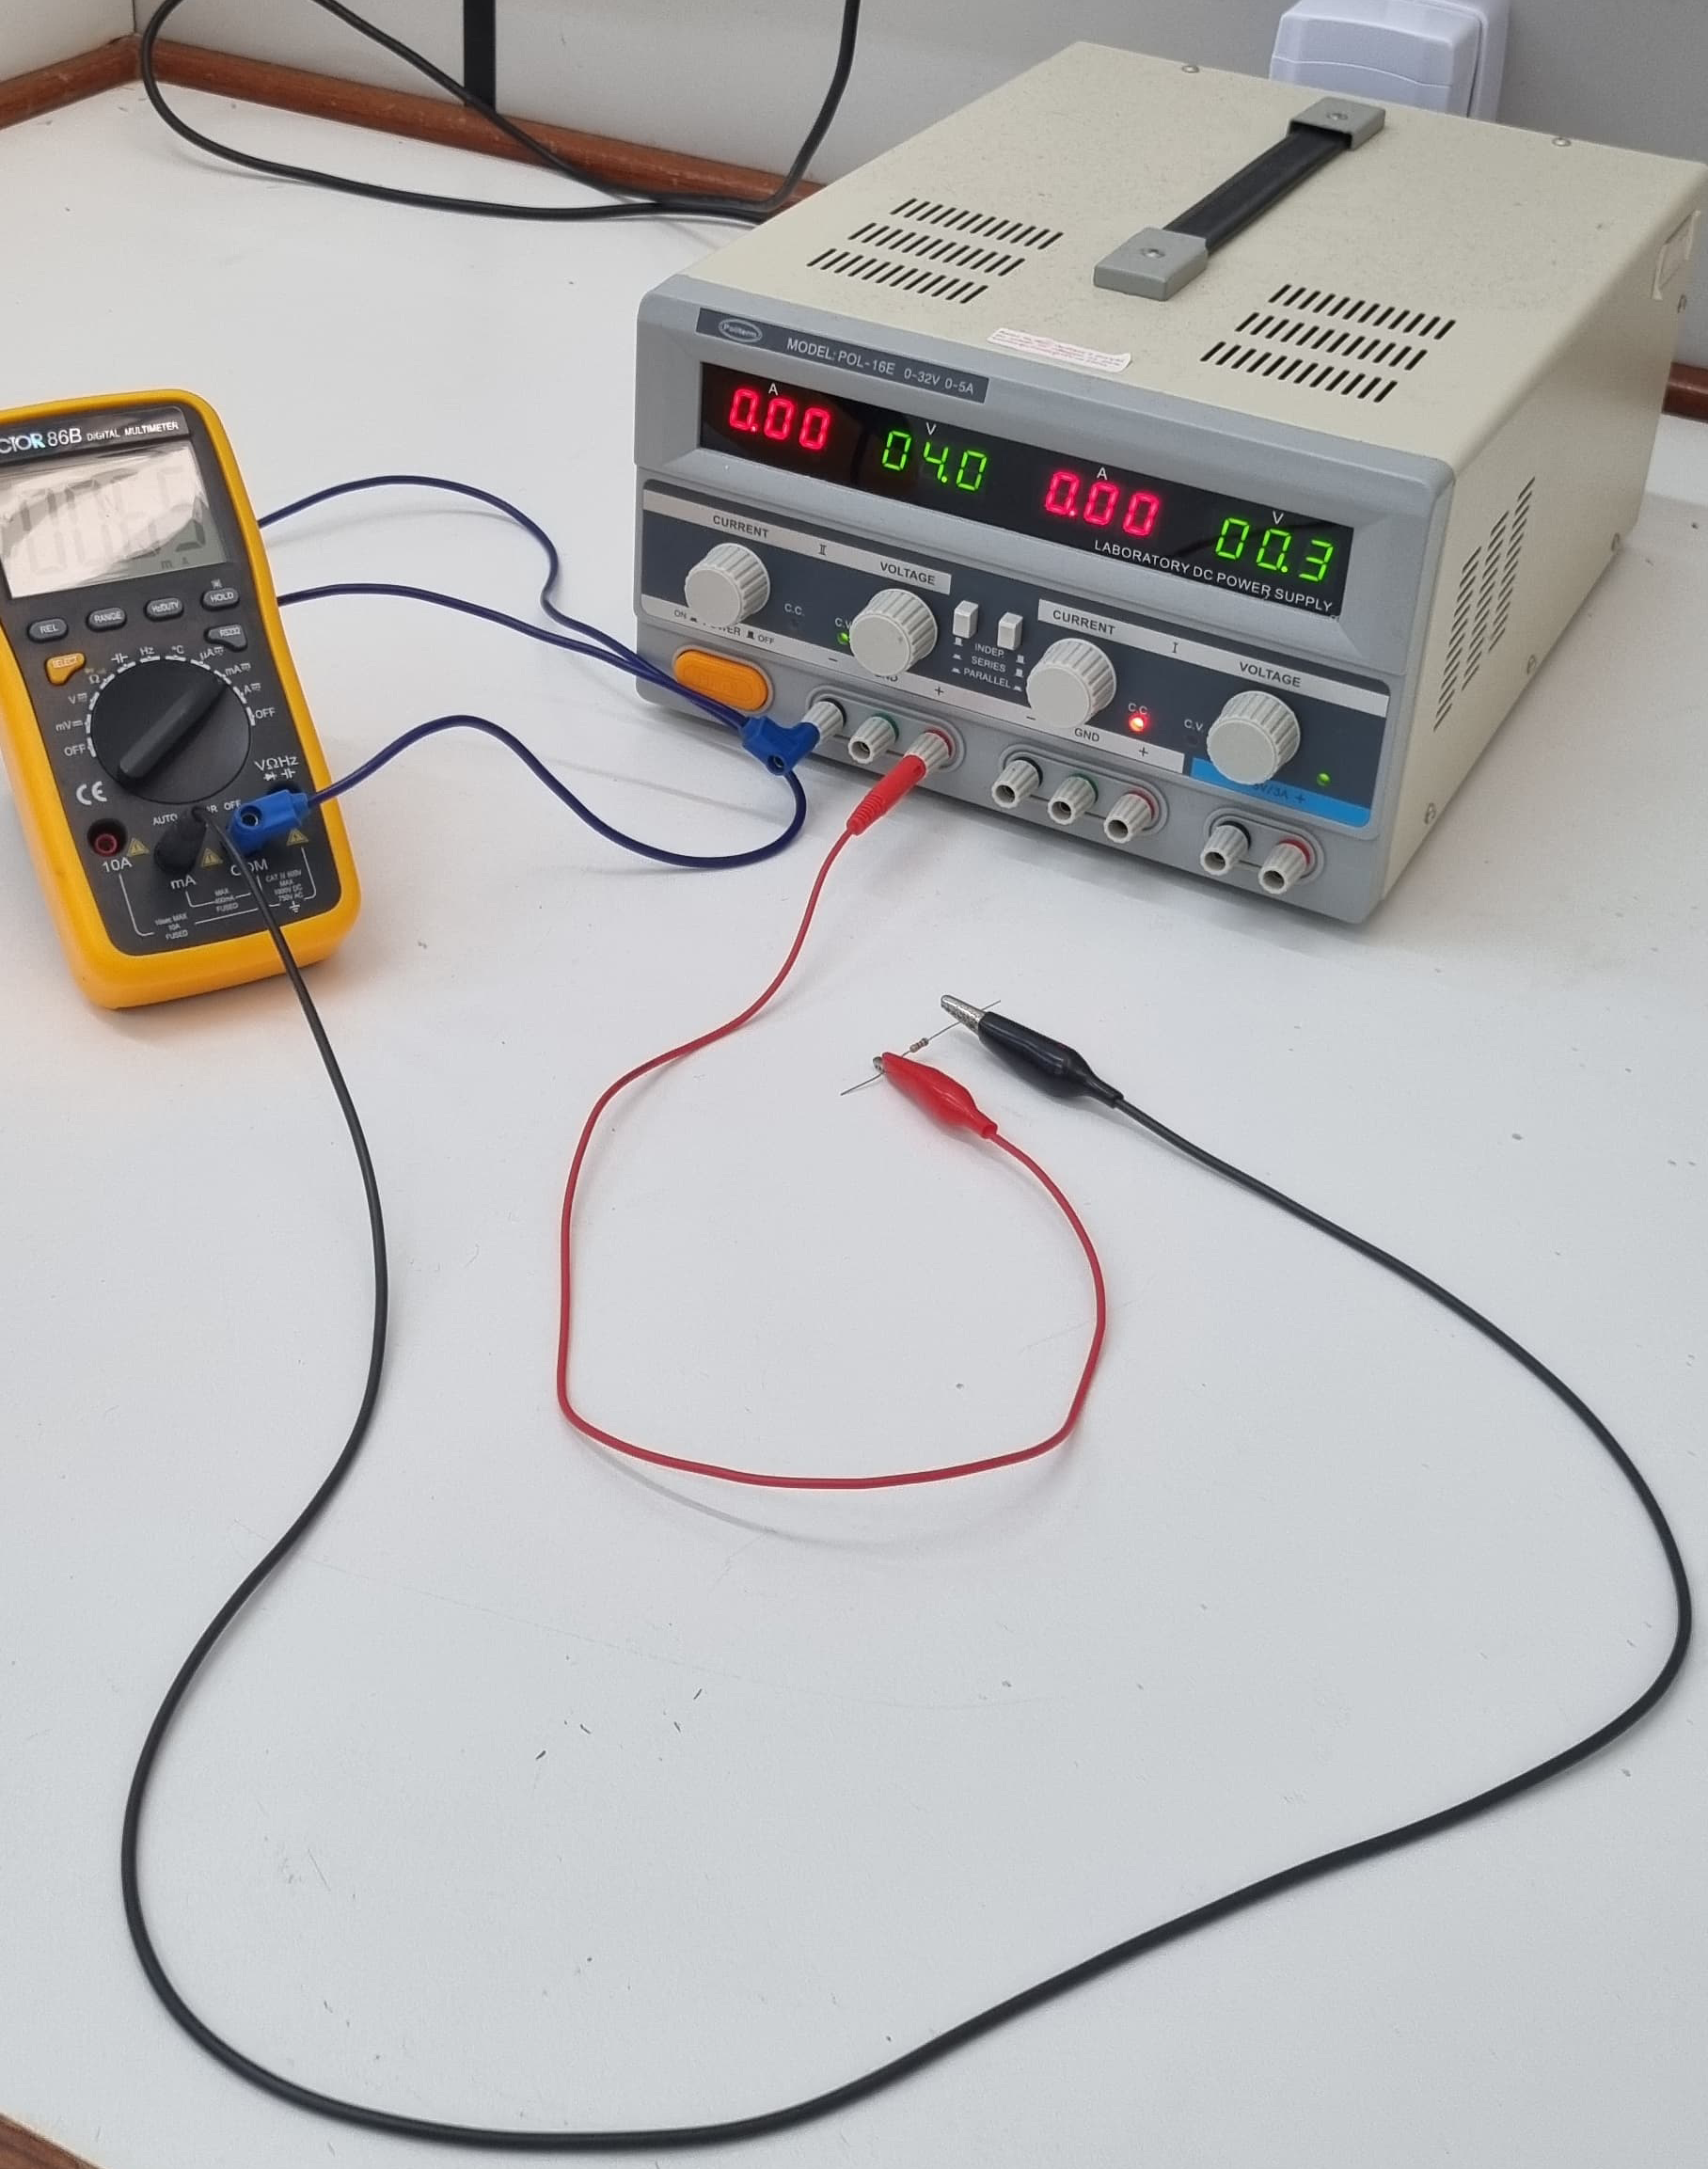
\includegraphics[width=\linewidth]{external-figures/circuito-pratica2.png}
    \end{subfigure}
    \label{fig:pratica-parte2}
\end{figure}

Então, variou-se a tensão, começando de 12 V até 0 V, e para cada tensão diferente mediu-se a corrente no respectivo resistor e anotou-a. Os resultados foram expressados na Tabela \ref{tab:corrente-fonte-variavel}.

\begin{table}[H]
    \caption{Corrente que passa por cada resistor conforme tensão.}
    \label{tab:corrente-fonte-variavel}
    \centering
    \setstretch{1.5}{
    \begin{tabular}{ccccc}
        \hline $R$     & 6,2 k$\Omega$ & 10 k$\Omega$ & 22 k$\Omega$ & 27 k$\Omega$ \\
        \hline $E$ (V) & $i_1$ (mA)    & $i_2$ (mA)   & $i_3$ (mA)   & $i_4$ (mA)   \\
        \hline 0       & 0,00          & 0,00         & 0,00         & 0,00         \\
        2              & 0,33          & 0,21         & 0,09         & 0,07         \\
        4              & 0,65          & 0,41         & 0,18         & 0,15         \\
        6              & 0,97          & 0,61         & 0,28         & 0,22         \\
        8              & 1,29          & 0,81         & 0,36         & 0,29         \\
        10             & 1,61          & 1,01         & 0,46         & 0,37         \\
        12             & 1,93          & 1,21         & 0,55         & 0,45         \\
        \hline
    \end{tabular}}\\
    \footnotesize{Fonte: Elaborado pelo autor.}
\end{table}

\subsubsection{Exercícios}
\textbf{1 - }Com os valores obtidos, levante o gráfico $V=f(i)$ para cada resistor.
\begin{figure}[H]
    \centering
    \caption{Resposta ao exercício 1.}
    \begin{subfigure}{0.45\textwidth}
        \centering
        \caption{$R_{6,2\text{k}\Omega}$}
        \begin{tikzpicture}[scale=0.7]
            \begin{axis}[
                axis lines=middle,
                xlabel={$i$ (mA)},
                ylabel={$V$ (V)},
                xlabel style = {at={(axis description cs:1.15,0)},anchor=south east},
                ylabel style = {at={(axis description cs:0,1)},anchor=south},
                xmin=-0.2, xmax=2.2,
                ymin=-2, ymax=14,
                xtick={0, 0.33, 0.65, 0.97, 1.29, 1.61, 1.93},
                xticklabels={0, 0.33, 0.65, 0.97, 1.29, 1.61, 1.93},
                ytick={0, 2, 4, 6, 8, 10, 12},
                yticklabels={0, 2, 4, 6, 8, 10, 12},
                x tick label style={rotate=45, anchor=east}
            ]
            \addplot coordinates {
                (0,0) (0.33,2) (0.65,4) (0.97,6) (1.29,8) (1.61,10) (1.93,12)
            };
            \node at (axis cs:0,0) [anchor=north east] {$0$};
            \end{axis}
        \end{tikzpicture}
    \end{subfigure}
    \hfill
    \begin{subfigure}{0.45\textwidth}
        \centering
        \caption{$R_{10\text{k}\Omega}$}
        \begin{tikzpicture}[scale=0.7]
            \begin{axis}[
                axis lines=middle,
                xlabel={$i$ (mA)},
                ylabel={$V$ (V)},
                xlabel style = {at={(axis description cs:1.15,0)},anchor=south east},
                ylabel style = {at={(axis description cs:0,1)},anchor=south},
                xmin=-0.2, xmax=1.75,
                ymin=-2, ymax=14,
                xtick={0, 0.21, 0.41, 0.61, 0.81, 1.01, 1.21},
                xticklabels={0, 0.21, 0.41, 0.61, 0.81, 1.01, 1.21},
                ytick={0, 2, 4, 6, 8, 10, 12},
                yticklabels={0, 2, 4, 6, 8, 10, 12},
                x tick label style={rotate=45, anchor=east}
            ]
            \addplot coordinates {
                (0,0) (0.21,2) (0.41,4) (0.61,6) (0.81,8) (1.01,10) (1.21,12)
            };
            \node at (axis cs:0,0) [anchor=north east] {$0$};
            \end{axis}
        \end{tikzpicture}
    \end{subfigure}

\vspace{\baselineskip}
    \begin{subfigure}{0.45\textwidth}
        \centering
        \caption{$R_{22\text{k}\Omega}$}
        \begin{tikzpicture}[scale=0.7]
            \begin{axis}[
                axis lines=middle,
                xlabel={$i$ (mA)},
                ylabel={$V$ (V)},
                xlabel style = {at={(axis description cs:1.15,0)},anchor=south east},
                ylabel style = {at={(axis description cs:0,1)},anchor=south},
                xmin=-0.08, xmax=0.75,
                ymin=-2, ymax=14,
                xtick={0, 0.09, 0.18, 0.28, 0.36, 0.46, 0.55},
                xticklabels={0, 0.09, 0.18, 0.28, 0.36, 0.46, 0.55},
                ytick={0, 2, 4, 6, 8, 10, 12},
                yticklabels={0, 2, 4, 6, 8, 10, 12},
                x tick label style={rotate=45, anchor=east}
            ]
            \addplot coordinates {
                (0,0) (0.09,2) (0.18,4) (0.28,6) (0.36,8) (0.46,10) (0.55,12)
            };
            \node at (axis cs:0,0) [anchor=north east] {$0$};
            \end{axis}
        \end{tikzpicture}
    \end{subfigure}
    \hfill
    \begin{subfigure}{0.45\textwidth}
        \centering
        \caption{$R_{27\text{k}\Omega}$}
        \begin{tikzpicture}[scale=0.7]
            \begin{axis}[
                axis lines=middle,
                xlabel={$i$ (mA)},
                ylabel={$V$ (V)},
                xlabel style = {at={(axis description cs:1.15,0)},anchor=south east},
                ylabel style = {at={(axis description cs:0,1)},anchor=south},
                xmin=-0.07, xmax=0.6,
                ymin=-2, ymax=14,
                xtick={0, 0.07, 0.15, 0.22, 0.29, 0.37, 0.45},
                xticklabels={0, 0.07, 0.15, 0.22, 0.29, 0.37, 0.45},
                ytick={0, 2, 4, 6, 8, 10, 12},
                yticklabels={0, 2, 4, 6, 8, 10, 12},
                x tick label style={rotate=45, anchor=east}
            ]
            \addplot coordinates {
                (0,0) (0.07,2) (0.15,4) (0.22,6) (0.29,8) (0.37,10) (0.45,12)
            };
            \node at (axis cs:0,0) [anchor=north east] {$0$};
            \end{axis}
        \end{tikzpicture}
    \end{subfigure}
    \label{fig:resposta-ex1}
\end{figure}

\noindent\textbf{2 - }Determine, por meio do gráfico, o valor de cada resistência.

O valor de cada resistência pode ser encontrado calculando a tangente do ângulo compreendido entre a reta mostrada e o eixo $i$, conforme a Equação \ref{lei-de-ohm}. Dessa forma:
\begin{align*}
    R_{6,2\text{k}\Omega}&=\frac{6}{0,97}= 6,19\ \text{k}\Omega \\
    R_{10\text{k}\Omega}&=\frac{6}{0,61}= 9,83\ \text{k}\Omega \\
    R_{22\text{k}\Omega}&=\frac{6}{0,28}= 21,43\ \text{k}\Omega \\
    R_{27\text{k}\Omega}&=\frac{6}{0,22}= 27,27\ \text{k}\Omega
\end{align*}

\noindent\textbf{3 - }Explique as discrepâncias dos valores nominais.

As discrepâncias nos valores nominais decorrem da tolerância que já vem de fábrica dos resistores, que no caso dos resistores utilizados foi de $\pm$5\%. Por exemplo, para um resistor nominal de 10 k$\Omega$, o valor real pode variar entre 9,5 k$\Omega$ e 10,5 k$\Omega$, mesmo antes de considerar os erros de medição. Além disso, a resistência interna do multímetro influencia a leitura da tensão nos terminais do resistor quando o circuito não é ideal. Essa influência é mais perceptível em medidores com maior resistência, nos quais a resistência interna altera o valor total do circuito, levando a leituras ligeiramente abaixo do esperado \parencite[][, p. 71]{nilsson}.

\section{CONCLUSÃO}
O experimento permitiu verificar a aplicação prática da Lei de Ohm, comprovando a relação linear entre tensão e corrente em resistores ôhmicos. Por meio das medições realizadas, foi possível observar pequenas discrepâncias entre os valores nominais e os valores medidos, explicadas pelas tolerâncias dos resistores e pelas limitações dos instrumentos utilizados. O uso de gráficos ajudou a ilustrar essas diferenças e demonstrou a importância de considerar as tolerâncias na análise de circuitos.

\newpage
\setstretch{1}
\section*{\hfill REFERÊNCIAS BIBLIOGRÁFICAS\hfill}
\addcontentsline{toc}{section}{REFERÊNCIAS BIBLIOGRÁFICAS}
\printbibliography[heading=none]
\end{document}